%                                                                 aa.dem
% AA vers. 9.1, LaTeX class for Astronomy & Astrophysics
% demonstration file
%                                                       (c) EDP Sciences
%-----------------------------------------------------------------------
%
%\documentclass[referee]{aa} % for a referee version
%\documentclass[onecolumn]{aa} % for a paper on 1 column  
%\documentclass[longauth]{aa} % for the long lists of affiliations 
%\documentclass[letter]{aa} % for the letters 
%\documentclass[bibyear]{aa} % if the references are not structured 
%                              according to the author-year natbib style

%
\documentclass{aa}  

%
\usepackage{graphicx}
%%%%%%%%%%%%%%%%%%%%%%%%%%%%%%%%%%%%%%%%
\usepackage{txfonts}
\usepackage[svgnames]{xcolor}
%%%%%%%%%%%%%%%%%%%%%%%%%%%%%%%%%%%%%%%%
% \usepackage[options]{hyperref}
% To add links in your PDF file, use the package "hyperref"
% with options according to your LaTeX or PDFLaTeX drivers.
%
\usepackage{hyperref}         % automagic cross-referencing
\usepackage{cleveref}
\newcommand\numberthis{\addtocounter{equation}{1}\tag{\theequation}}
% defines the color of hyperref objects
% Blending two colors:  blue!80!black  =  80% blue and 20% black
\hypersetup{ % this is just my personal choice, feel free to change things
    colorlinks,
    linkcolor={red!50!black},
    citecolor={blue!20!purple!80!black},
    urlcolor={blue!80!black},
    breaklinks=true}
\urlstyle{same}
\begin{document} 


   \title{TITLE}

   \subtitle{AST5220}

   \author{Håvard Skåli
        %   \inst{1}
          }

   \institute{Institute of Theoretical Astrophysics (ITA), University of Oslo}

   \date{\today}

% \abstract{}{}{}{}{} 
% 5 {} token are mandatory
 
  \abstract

  {}
  {AIMS}
  {METHODS}
  {RESULTS}
  {}\keywords{KEYWORDS}

   \maketitle
%
%-------------------------------------------------------------------
\section{Introduction}\label{sec: introduction}
\colorbox{Plum}{mention here that we use Planck 2018} \\
\colorbox{Plum}{mention that theory is from the website}

\section{Milestone I}\label{sec: milestone I}
The evolution of the universe is governed by the interplay between different energy components, including radiation, matter, and dark energy. Understanding how these components influence the expansion history is essential for predicting the large-scale structure of the Universe and the Cosmic Microwave Background (CMB) fluctuations. This milestone focuses on modeling the background evolution of the universe using the Friedmann equations, which describe how the Hubble parameter $H$, and thus time and distance measures, evolve with redshift. I will implement a numerical framework that takes in cosmological parameters and computes such key background quantities, and use this to fit to measurements of supernova luminosity distances. \colorbox{Plum}{word differently?} My approach involves numerically solving the Friedmann equations and interpolating the results using splines to extract meaningful physical insights.

By completing this milestone, the goal is to establish a robust computational framework that will serve as the foundation for later stages of the project, where I will analyze perturbations and extract information about the CMB anisotropies. The results from this milestone will therefore be essential for constraining cosmological parameters using observational data.

\subsection{Theory}\label{subsec: I theory}
\subsubsection{Evolution of the Universe and the Hubble parameter}
The expansion of the Universe is governed by General Relativity, with the large-scale dynamics described by the Friedmann-Lemaître-Robertson-Walker (FLRW) metric. Assuming a homogeneous and isotropic universe, the metric is given by
\begin{equation}
    ds^2 = -c^2 dt^2 + a^2(t) \left[ \frac{dr^2}{1 - k r^2} + r^2 d\theta^2 + r^2 \sin^2\theta d\phi^2 \right],
\end{equation}
where $a(t) = 1/(1+z)$ is the dimensionless scale factor, with $z$ being the cosmological redshift. The constant $k$ determines the curvature of the Universe ($k = 0$ for a flat universe, $k > 0$ for a closed universe, and $k < 0$ for an open universe). \colorbox{Plum}{explain scaling of a?}

The evolution of $a(t)$ is governed by the Friedmann equation, which is derived from Einstein's field equations: \colorbox{Plum}{cite notes?}
\begin{equation}
    H^2 = \frac{8\pi G}{3} \sum_{i}\rho_i - \frac{k c^2}{a^2} \simeq \frac{8\pi G}{3} \sum_{i}\rho_i,
\end{equation}
Here, $H = \dot{a}/a$ is the Hubble parameter, and $\rho_i$ denotes the total energy density of some component (photons, baryons, etc.). In the second equality I have used that we can treat the curvature as its own component that is included in the sum, with energy density
\begin{equation}
  \rho_k = -\frac{3}{8\pi G}\frac{k c^2}{a^2}. \label{eq:rho k}
\end{equation}
It is essential to know not only how the curvature ``energy density'' scales with $a$, but the other components as well. To understand this, we start with the continuity equation for a perfect fluid, which is a very accurate description of the energy density components in the Universe on the largest scales, applied to a homogeneous and isotropic universe:
\begin{equation}
  \frac{d\rho}{dt} + 3H (\rho_i+ p_i) = \frac{d\rho}{dt} + \frac{3}{a}\frac{da}{dt} \rho_i(1 + w_i) = 0.
\end{equation}
Here, $p_i$ is the pressure of the fluid, and $w_i=p_i/\rho_i$ is the equation of state parameter, which is constant for the fluids considered in conventional cosmology. This differential equation is easily solved by separating variables and integrating, which gives us:
\begin{equation}
  \rho_i(a) = \rho_{i0} a^{-3(1+w_i)},
\end{equation}
where $\rho_{i0}$ is the present-day density.

On universal scales, non-relativistic matter can essentially be treated as pressureless, hence $w_m = w_b=w_\text{CDM}=0$ and thus $\rho_m \propto a^{-3}$. This corresponds to the dilution of a density field in an expanding volume. Furthermore, neutrinos are so light that they can still be treated as relativistic (radiation), and we therefore have $w_r=w_\gamma=w_\nu=1/3$, which implies $\rho_r\propto a^{-4}$. Radiation is also diluted as the Universe expands, and the extra factor of $a^{-1}$ comes from redshifting of relativistic particles in an expanding universe. From eq. \eqref{eq:rho k} we indeed see that we can treat curvature as a perfect fluid with equation of state $w_k=-1/3$, while dark energy, represented by the cosmological constant $\Lambda$, remains constant in time, hence $w_\Lambda=-1$.

A much more convenient way of writing the Friedmann equation can be derived by defining the critical density, which is the density required for a flat universe ($k=0$):
\begin{equation}
  \rho_c = \frac{3 H^2}{8 \pi G}.
\end{equation}
We may then define the dimensionless density parameters, which describe how much of the total energy density each component $i$ contributes:
\begin{equation}
  \Omega_i = \frac{\rho_{i}}{\rho_c}.
\end{equation}
Substituting this into the Friedmann equation gives us then
\begin{equation}
  H^2 = \frac{8\pi G}{3} \sum_i \Omega_{i}\rho_c = H^2\sum_i \Omega_{i}, \label{eq:H squared}
\end{equation}
which shows us explicitly that the density parameters always must sum up to unity. We would like to rewrite this in terms of quantities that we can actually measure today, such as the present day density parameters $\Omega_{i0}$. In that case, $H^2$ becomes $H_0^2$ on the right-hand side of eq. \eqref{eq:H squared}. Furthermore, since we know how the density components scale with $a$, we may write
\begin{equation}
  H^2 = H_0^2\sum_i \Omega_{i0}a^{-3(1+w_i)}. \label{eq:H squared 2}
\end{equation} 
The equivalency of this expression with eq. \eqref{eq:H squared} tells us that
\begin{equation}
  \Omega_{i}(a) = \frac{\Omega_{i0}a^{-3(1+w_i)}}{H^2(a)/H_0^2}, \label{eq:density params}
\end{equation}
Additionally, taking the square root on both sides of eq. \eqref{eq:H squared 2} and writing out the terms explicitly, we have
\begin{equation}
    H = H_0 \sqrt{(\Omega_{b0} + \Omega_{\text{CDM}0}) a^{-3} + (\Omega_{\gamma 0} + \Omega_{\nu 0}) a^{-4} + \Omega_{k0} a^{-2} + \Omega_{\Lambda 0}}.
\end{equation}

Eventually, I will need to use data to determine all but the photon and neutrino density parameters, which we know are given by
\begin{align}
    \Omega_{\gamma0} &= g\frac{\pi^2}{30}\frac{\left(k_\text{B}T_{\text{CMB}0}\right)^4}{\hbar^3c^5}\frac{8\pi G}{3H_0^2},
    \\
    \Omega_{\nu0} &= \frac{7}{8}N_\text{eff}\left(\frac{4}{11}\right)^{1/3}\Omega_{\gamma0}.
\end{align}
Here, $g=g_\gamma=g_\nu=2$, since photons and neutrinos both have 2 internal polarization states, while $T_{\text{CMB}0}$ is the present day value of the CMB temperature, and $N_\text{eff}$ is the effective number of relativistic degrees of freedom. 
% Together with the baryon ($\Omega_{b0}$), cold dark matter ($\Omega_{\text{CDM}0}$) and curvature ($\Omega_{k0}$) density parameters, we then get the dark energy density parameter from
% \begin{equation}
%     \Omega_{\Lambda0} = 1 - \left(\Omega_{k0} + \Omega_{b0} + \Omega_{\text{CDM}0} + \Omega_{\gamma0} + \Omega_{\nu0} \right),
% \end{equation}
% since the density parameters must all sum to unity. 

When integrating from the very early universe, it becomes quite numerically challenging to use the scale factor $a$ as time parameter, as it quickly tends to vanishing orders of magnitude as we move further back in time. \colorbox{Plum}{rephrase?}, I will therefore adopt the logarithmic time coordinate
\begin{equation}
    x = \log a,
\end{equation}
instead, which implies that $x=0$ today and $x=-\infty$ at the Big Bang. Expressed in terms of $\Omega_{m0}=\Omega_{b0}+\Omega_{\text{CDM}0}$ and $\Omega_{r0}=\Omega_{\gamma0}+\Omega_{\nu0}$, we can equivalently write the Hubble parameter as
\begin{equation}
    H = H_0 \sqrt{\Omega_{m0} e^{-3x} + \Omega_{r0} e^{-4x} + \Omega_{k0} e^{-2x} + \Omega_{\Lambda 0}}.
\end{equation}

A commonly used rescaled version of the Hubble parameter is the conformal Hubble parameter:
\begin{equation}
    \mathcal{H} = aH = H_0 \sqrt{\Omega_{m0} e^{-x} + \Omega_{r0} e^{-2x} + \Omega_{k0} + \Omega_{\Lambda 0}e^{2x}}. \label{eq:Hp}
\end{equation}
This naturally appears when rewriting cosmological equations in terms of the conformal time $\eta$, which I will present below. \colorbox{Plum}{explain why?} I will focus more on this version of the Hubble parameter, and it will become useful to know its first and second derivatives with respect to $x$, specifically in order to verify numerical stability. \colorbox{Plum}{explain why?} After some tedious calculation, we find that these are
\begin{align*}
    \frac{d\mathcal{H}}{dx} &= \frac{H_0}{2}
    \frac{-\Omega_{m0}e^{-x} - 2\Omega_{r0}e^{-2x} + 2\Omega_{\Lambda0}e^{2x}}
    {\sqrt{\Omega_{m0}e^{-x} 
    + \Omega_{r0}e^{-2x}
    + \Omega_{k0} + \Omega_{\Lambda0}e^{2x}}},
    \\
    &= -\frac{H_0^2}{2\mathcal{H}}\left(\Omega_{m0}e^{-x} + 2\Omega_{r0}e^{-2x} - 2\Omega_{\Lambda0}e^{2x}\right), \numberthis
    \\
    \frac{d^2\mathcal{H}}{dx^2} &= \frac{H_0}{2}
    \left(\frac{\Omega_{m0}e^{-x} + 4\Omega_{r0}e^{-2x} + 4\Omega_{\Lambda0}e^{2x}}{\sqrt{\Omega_{m0}e^{-x} + \Omega_{r0}e^{-2x} + \Omega_{k0} + \Omega_{\Lambda0}e^{2x}}}\right.
    \\
    &\hspace{38pt}
    \left.- \frac{1}{2}\frac{\left(\Omega_{m0}e^{-x} + 2\Omega_{r0}e^{-2x} - 2\Omega_{\Lambda0}e^{2x}\right)^2}{\left(\Omega_{m0}e^{-x} + \Omega_{r0}e^{-2x} + \Omega_{k0} + \Omega_{\Lambda0}e^{2x}\right)^{3/2}}\right),
    \\
    &= \frac{H_0^2}{\mathcal{H}}\left[\frac{1}{2}\Omega_{m0}e^{-x} + 2\Omega_{r0}e^{-2x} + 2\Omega_{\Lambda0}e^{2x}- \frac{1}{H_0^2}\left(\frac{d\mathcal{H}}{dx}\right)^2\right]. \numberthis
  \end{align*}


\subsubsection{Conformal time and distance measures}
The cosmic time $t$ is related to our time variable $x$ through
\begin{equation}
  \frac{dt}{dx} = \frac{dt}{da}\frac{da}{dx} = \frac{a}{\dot{a}} = \frac{1}{H},
\end{equation}
hence, to compute the cosmic time $t$ given our time coordinate $x$, we simply integrate this to get 
\begin{equation}
  t(x) = \int_{-\infty}^{x} \frac{dx'}{H(x')}.
\end{equation}
Evaluating this at $x=0$ (today), we obtain the age of the Universe.

While it will be interesting to solve our system of equations for $t$, it will be more useful to introduce the conformal time $\eta$. This is defined as
\begin{equation}
d\eta = \frac{cdt}{a} \hspace{5pt}\Leftrightarrow\hspace{5pt}\frac{d\eta}{dx} = \frac{c}{\mathcal{H}},
\end{equation}
and thus has units of length. The equation on the right can easily be numerically integrated to obtain $\eta(x)$, which describes how far light has traveled since the Big Bang. In other words, the comoving distance a photon has traveled since the start of the Universe is given by:
\begin{equation}
\chi = \eta_0 - \eta,
\end{equation}
where $\eta_0$ is the conformal time today. This quantity is also called the particle horizon, and it is a crucial concept in cosmology, as it represents the maximum comoving distance that light has traveled since the beginning of the Universe, thus determining its causal structure. 

The horizon is fundamental in defining distance measures in cosmology. We know that photons travel along null geodesics $ds^2 = 0$, and from the conformal time and the FLRW line element we see that this implies that the coordinate distance $r$ satisfies
\begin{equation}
  c dt = \frac{adr}{\sqrt{1 - k r^2}},
\end{equation}
for a radially traveling photon ($d\theta = d\phi = 0$). Changing the time coordinate to conformal time, we rewrite this as
\begin{equation}
  d\eta = \frac{dr}{\sqrt{1 - k r^2}},
\end{equation}
and integrating from emission at time $\eta$ to today (\( \eta_0 \)), we get the comoving distance:
\begin{equation}
  \chi = \int_{\eta}^{\eta_0}  d\eta' = \int_{0}^{r} \frac{dr'}{\sqrt{1 - k r'^2}}.
\end{equation}
Solving this integral for different values of the curvature constant $k$, we obtain
\begin{equation}
  r = 
  \chi\begin{cases}
  \cfrac{\sin\left(\sqrt{|\Omega_{k0}|} H_0 \chi / c\right)}{\left(\sqrt{|\Omega_{k0}|} H_0 \chi / c\right)}, & \Omega_{k0} < 0 \quad \text{(Closed)}, \\
1, & \Omega_{k0} = 0 \quad \text{(Flat)}, \\
\cfrac{\sinh\left(\sqrt{|\Omega_{k0}|} H_0 \chi / c\right)}{\left(\sqrt{|\Omega_{k0}|} H_0 \chi / c\right)}, & \Omega_{k0} > 0 \quad \text{(Open)}.
\end{cases}
\end{equation}
This defines the proper radial coordinate $r$, which is used in all cosmological distance measures. 

The angular diameter distance relates an object's physical extent $D$ to its observed angular extent $\theta$ on the sky:
\begin{equation}
d_A = \frac{D}{\theta}.
\end{equation}
From the metric, we see that the transverse separation of a source at $r$ subtending an angle $d\theta$ is
\begin{equation}
  dD = a r d\theta,
\end{equation}
hence the angular diameter distance:
\begin{equation}
  d_A = a r,
\end{equation}
which simplifies to:
\begin{equation}
  d_A = a \chi,
\end{equation}
for a flat universe.

Even more relevant for this milestone is the luminosity distance, which is dependent on the measured brightness of standard candles like Type Ia supernovae. We know that the flux $F$ from a source with luminosity $L$ follows an inverse-square law:
\begin{equation}
  F = \frac{L}{4\pi d_L^2}.
\end{equation}
In an expanding universe, photons are redshifted and their arrival rate is also affected, leading to the relation:
\begin{equation}
  d_L = d_A (1 + z)^2 = \frac{d_A}{a^2}.
\end{equation}
\colorbox{Plum}{TODO: maybe explain}



\subsubsection{Key cosmological epochs}
Though it also has been verified by numerous observations, based on the expression for the Hubble parameter it is not hard to see that the Universe must have gone through phases where its energy budget was (or will be) dominated by radiation, matter and dark energy, separately, in that order. This implies that there must have been a point in time where the Universe was equal amounts of radiation and matter (matter and dark energy), if we neglect the curvature and dark energy (radiation). At radiation-matter equality ($rm$) we have
\begin{equation}
    \Omega_{r,rm} = \Omega_{m,rm} 
    \hspace{5pt}\Leftrightarrow\hspace{5pt} 
    \Omega_{r0}e^{-4x_{rm}} = \Omega_{m0}e^{-3x_{rm}}, 
\end{equation}
and thus
\begin{equation}
  x_{rm} = \log\left(\frac{\Omega_{r0}}{\Omega_{m0}}\right).
\end{equation}
Using that $x = \log a$ and $z = 1/a - 1$ this gives us an expression for the redshift at $rm$:
\begin{equation}
  z_{rm} = \frac{\Omega_{m0}}{\Omega_{r0}} - 1.
\end{equation} 
Similarly, at matter-dark energy equality ($m\Lambda$) we have
\begin{equation}
  \Omega_{m0}e^{-3x_{m\Lambda}} = \Omega_{\Lambda0}
  \hspace{5pt}\Leftrightarrow\hspace{5pt}
  x_{m\Lambda} = \frac{1}{3}\log\left(\frac{\Omega_{m0}}{\Omega_{\Lambda0}}\right),
\end{equation}
and thus
\begin{equation}
  z_{m\Lambda} = \left(\frac{\Omega_{\Lambda0}}{\Omega_{m0}}\right)^{1/3} - 1.
\end{equation}

To ensure that the numerical results presented in this work agree with analytical expectations, it will be beneficial to have approximate expressions for the cosmic and conformal times in the different regimes. For a universe dominated by a single component with equation of state $w_i$ the cosmic time $t$ is given by
\begin{equation}
  t = \int_0^t dt' = \int_{-\infty}^{x}\frac{dx'}{H_0\sqrt{\Omega_{i0}e^{-3(1+w_i)x'}}}.
\end{equation}
When the Universe transitions between an era where its energy density is dominated by some component $\rho_j$ to some other component $\rho_i$, we may neglect all other components and compute an approximate expression for the cosmic time as function of $x$ by writing
\begin{equation}
  t_i(x) \approx t_{j,i} + \int_{x_{j,i}}^{x}\frac{dx'}{H_0\sqrt{\Omega_{i0}e^{-3(1+w_i)x'}}},
\end{equation}
where $x_{j,i}$ and $t_{j,i}$ correspond to their values when $\rho_j=\rho_i$. For radiation we simply have $x_{j,i}=-\infty$ and thus $t_{j,i}=0$, since the very early Universe was filled with relativistic particles, hence
\begin{equation}
  t_r(x) = \int_{{-\infty}}^{x}\frac{dx'}{H_0\sqrt{\Omega_{r0}e^{-4x'}}} = \frac{1}{2H_0\sqrt{\Omega_{r0}e^{-4x}}}.
\end{equation}
We see that radiation-matter equality occurs at
\begin{equation}
  t_{rm} = t_r(x_{rm}) = \frac{\Omega_{r0}^{3/2}}{2H_0\Omega_{m0}^2},
\end{equation}
and for matter it then follows
\begin{align*}
  t_m(x) &\approx t_{rm} + \int_{x_{rm}}^{x}\frac{dx'}{H_0\sqrt{\Omega_{m0}e^{-3x'}}}, 
  \\
  &= \frac{\Omega_{r0}^{3/2}}{2H_0\Omega_{m0}^2}+\frac{2}{3H_0}\left[\frac{1}{\sqrt{\Omega_{m0}e^{-3x}}} - \frac{\Omega_{r0}^{3/2}}{H_0\Omega_{m0}^2} \right],
  \\
  &= \frac{1}{3H_0}\left[\frac{2}{\sqrt{\Omega_{m0}e^{-3x}}} - \frac{\Omega_{r0}^{3/2}}{2\Omega^2_{m0}} \right], \numberthis
\end{align*}
with matter-dark energy equality occuring at
\begin{equation}
  t_{m\Lambda} = \frac{1}{3H_0}\left[\frac{2}{\sqrt{\Omega_{\Lambda0}}} - \frac{\Omega_{r0}^{3/2}}{2\Omega^2_{m0}} \right].
\end{equation}
Lastly, for dark energy we have
\begin{align*}
  t_\Lambda(x) &\approx t_{m\Lambda} + \int_{x_{m\Lambda}}^{x}\frac{dx'}{H_0\sqrt{\Omega_{\Lambda0}}}, 
  \\
  &= \frac{1}{3H_0}\left[\frac{2}{\sqrt{\Omega_{\Lambda0}}} - \frac{\Omega_{r0}^{3/2}}{2\Omega^2_{m0}} \right] + \frac{1}{H_0\sqrt{\Omega_{\Lambda0}}}\left[x - \frac{1}{3}\log\left(\frac{\Omega_{m0}}{\Omega_{\Lambda0}}\right)\right],
  \\
  &= \frac{1}{H_0\sqrt{\Omega_{\Lambda0}}}\left[x+\frac{2}{3}-\frac{1}{3}\log\left(\frac{\Omega_{m0}}{\Omega_{\Lambda0}}\right)-\frac{\sqrt{\Omega_{\Lambda0}}\Omega_{r0}^{3/2}}{6\Omega^2_{m0}}\right]. \numberthis
\end{align*}
From these derived expressions, it is obvious that $a\propto t^{1/2}$ in the radiation dominated era, $a\propto t^{2/3}$ in the matter era and $a\propto e^{H_0\sqrt{\Omega_{\Lambda0}}t}$ in the dark energy era, which is the expected result. \colorbox{Plum}{word different?}

Following an analogous approach for the conformal time, it is straight-forward to show that since
\begin{equation}
  \eta_i(x) \approx \eta_{j,i} + \int_{x_{j,i}}^{x}\frac{cdx'}{H_0\sqrt{\Omega_{i0}e^{-(1+3w_i)x'}}},
\end{equation}
we have the following approximate expressions:
\begin{align}
  \eta_r(x) &= \frac{c}{H_0\sqrt{\Omega_{r0}e^{-2x}}},
  \\
  \eta_m(x) &= \frac{c}{H_0}\left[\frac{2}{\sqrt{\Omega_{m0}e^{-x}}} - \frac{\sqrt{\Omega_{r0}}}{\Omega_{m0}} \right],
  \\
  \eta_\Lambda(x) &= -\frac{c}{H_0}\left[\frac{1}{\sqrt{\Omega_{\Lambda0}e^{2x}}} +\frac{\sqrt{\Omega_{r0}}}{\Omega_{m0}} - \frac{3}{\Omega_{m0}^{1/3}\Omega_{\Lambda0}^{1/6}} \right],
\end{align}
with the conformal equality times:
\begin{align}
  \eta_{rm} &= \frac{c}{H_0}\frac{\sqrt{\Omega_{r0}}}{\Omega_{m0}},
  \\
  \eta_{m\Lambda} &= \frac{c}{H_0}\left[\frac{2}{\Omega_{m0}^{1/3}\Omega_{\Lambda0}^{1/6}} - \frac{\sqrt{\Omega_{r0}}}{\Omega_{m0}}\right].
\end{align}

To test for numerical stability and accuracy, it is essential to compute analytical expressions that can be used for comparison. Obviously, in an era dominated by component $i$ we have
\begin{equation}
    \mathcal{H}_i \approx H_0\sqrt{\Omega_{i0}e^{-(1+3w_i)}},
\end{equation}
and in the radiation dominated era we thus have
\begin{align}
  \left(\frac{d\mathcal{H}}{dx}\right)_r &= -H_0\sqrt{\Omega_{r0}}e^{-x}=-\mathcal{H}_r 
  \hspace{5pt}\Leftrightarrow\hspace{9pt}\left(\frac{1}{\mathcal{H}}\frac{d\mathcal{H}}{dx}\right)_r=-1,
  \\
  \left(\frac{d^2\mathcal{H}}{dx^2}\right)_r &= H_0\sqrt{\Omega_{r0}}e^{-x}=\mathcal{H}_r
  \hspace{18pt}\Leftrightarrow\hspace{5pt}\left(\frac{1}{\mathcal{H}}\frac{d^2\mathcal{H}}{dx^2}\right)_r=1.
\end{align}
Similarly, we have
\begin{align}
  \left(\frac{d\mathcal{H}}{dx}\right)_m &= -\frac{\mathcal{H}_m}{2} 
  \hspace{5pt}\Leftrightarrow\hspace{10pt}\left(\frac{1}{\mathcal{H}}\frac{d\mathcal{H}}{dx}\right)_m=-\frac{1}{2},
  \\
  \left(\frac{d^2\mathcal{H}}{dx^2}\right)_m &= \frac{\mathcal{H}_m}{4}
  \hspace{12pt}\Leftrightarrow\hspace{5pt}\left(\frac{1}{\mathcal{H}}\frac{d^2\mathcal{H}}{dx^2}\right)_m=\frac{1}{4}.
\end{align}
in the matter dominated era, and
\begin{equation}
  \mathcal{H}_\Lambda = \left(\frac{d\mathcal{H}}{dx}\right)_\Lambda = \left(\frac{d^2\mathcal{H}}{dx^2}\right)_\Lambda = H_0\sqrt{\Omega_{\Lambda0}}e^{x},
\end{equation}
in the dark energy dominated era. From the latter it is obvious that
\begin{equation}
  \left(\frac{1}{\mathcal{H}}\frac{d\mathcal{H}}{dx}\right)_\Lambda = \left(\frac{1}{\mathcal{H}}\frac{d^2\mathcal{H}}{dx^2}\right)_\Lambda = 1.
\end{equation} 


\subsubsection{Onset of acceleration}
Later on, when we will analyze the observed CMB power spectrum, it will be interesting to know when the expansion of the Universe started to accelerate. It is a well known fact that the expansion rate (governed by $\dot{a}$) is increasing as of today, and that we are in the early stage of a dark energy dominated era. We have the second Friedmann equation
\begin{equation}
    \frac{\ddot{a}}{a} = -\frac{4\pi G}{3}\sum_i \rho_i\left(1 + 3w_i \right),
\end{equation}
where the sum runs over all components (matter, radiation, etc.). The onset of acceleration occurs when $\ddot{a}$ switches sign, i.e., when
\begin{equation}
    \sum_i \rho_i\left(1 + 3w_i \right) = 0.
\end{equation}
Assuming that this happens well after the radiation dominated era, we can approximate this as
\begin{equation}
  \rho_m(x_\text{acc})- 2\rho_\Lambda(x_\text{acc}) = 0 \label{eq: equal acc time}
\end{equation}
Using that the expression \eqref{eq:density params} for the density parameters at arbitrary $a$, we can rewrite eq. \eqref{eq: equal acc time} to get
\begin{equation}
  \Omega_{m0}e^{-3x_\text{acc}} = 2\Omega_{\Lambda0}
  \hspace{5pt}\Leftrightarrow\hspace{5pt}
  x_\text{acc} = \frac{1}{3}\log\left(\frac{\Omega_{m0}}{2\Omega_{\Lambda0}}\right).
\end{equation}
This corresponds to a redshift
\begin{equation}
  z_\text{acc} = \left(\frac{2\Omega_{\Lambda0}}{\Omega_{m0}}\right)^{1/3}-1.
\end{equation}
Obviously, $t_\text{acc}<t_{m\Lambda}$, so we can make the same approximation this time, hence
% \begin{equation}
%   t_\text{acc} = t_{rm} + \int^{x_\text{acc}}_{x_{rm}}\frac{dx}{H_0\sqrt{\Omega_{m0}e^{-3x}}} = \frac{1}{3H_0}\left(\sqrt{\frac{2}{\Omega_{\Lambda0}}} -\frac{\Omega_{r0}^{3/2}}{2\Omega_{m0}^2}\right).
% \end{equation}
\begin{equation}
    t_\text{acc} = t_m(x_\text{acc}) = \frac{1}{3H_0}\left[\sqrt{\frac{2}{\Omega_{\Lambda0}}} -\frac{\Omega_{r0}^{3/2}}{2\Omega_{m0}^2}\right],
\end{equation}
with the conformal time being
\begin{equation}
    \eta_\text{acc} = \eta_m(x_\text{acc}) = \frac{c}{H_0}\left[\frac{2^{5/6}}{\Omega_{m0}^{1/3}\Omega_{\Lambda0}^{1/6}} - \frac{\sqrt{\Omega_{r0}}}{\Omega_{m0}}\right].
\end{equation}
\colorbox{Plum}{maybe do this derivation more thorough/different}

\subsubsection{The Universe today}
It is of course a great consistency check to see if I am able to replicate the values for the age of the Universe and its horizon size today, and we can use the expressions derived above to do so. Following the approximations I have done up until this point, we have
\begin{align}
  t_0 &\approx t_{\Lambda}(0) = \frac{1}{H_0\sqrt{\Omega_{\Lambda0}}}\left[\frac{2}{3}-\frac{1}{3}\log\left(\frac{\Omega_{m0}}{\Omega_{\Lambda0}}\right)-\frac{\sqrt{\Omega_{\Lambda0}}\Omega_{r0}^{3/2}}{6\Omega^2_{m0}}\right],
  \\
  \eta_0 &\approx \eta_\Lambda(0) = -\frac{c}{H_0}\left[\frac{1}{\sqrt{\Omega_{\Lambda0}}} +\frac{\sqrt{\Omega_{r0}}}{\Omega_{m0}} - \frac{3}{\Omega_{m0}^{1/3}\Omega_{\Lambda0}^{1/6}} \right].
\end{align}
as we know that we currently are in the beginning of a dark energy dominated era.

\colorbox{Plum}{maybe remove and present in results}


\subsubsection{The \texorpdfstring{$\chi^2$}{Lg}-method}
\color{Plum}
Having established the theoretical framework describing the evolution of the universe, we now turn to how observational data can be used to constrain cosmological parameters. One of the most powerful tools for this is the study of Type Ia supernovae, which serve as standard candles for measuring the expansion history of the universe. Given their intrinsic luminosity, the observed flux allows us to determine their luminosity distance \( d_L \) as a function of redshift \( z \), providing a direct probe of the universe's geometry and expansion.

To quantitatively compare theoretical models to observational data, we define the chi-squared statistic:

\[
\chi^2(h, \Omega_{m0}, \Omega_{k0}) = \sum_{i=1}^{N} \frac{ \left( d_L(z_i, h, \Omega_{m0}, \Omega_{k0}) - d_L^{\text{obs}}(z_i) \right)^2 }{\sigma_i^2},
\]

where \( d_L^{\text{obs}}(z_i) \) represents the measured luminosity distance at redshift \( z_i \), and \( \sigma_i \) is the associated measurement uncertainty. This function quantifies how well a given set of parameters \( (h, \Omega_{m0}, \Omega_{k0}) \) fits the data: a lower \( \chi^2 \) value corresponds to a better fit. 

The likelihood function, describing the probability of the data given a specific model, is proportional to:

\[
L \propto e^{-\chi^2/2}.
\]

Rather than exhaustively evaluating \( \chi^2 \) over all parameter combinations, which is computationally expensive, we employ a Monte Carlo Markov Chain (MCMC) approach, such as the Metropolis-Hastings algorithm. This method efficiently samples the likelihood distribution, generating a chain of parameter values that follow the posterior probability distribution. 

From this chain, we determine the best-fit model—the parameter set yielding the minimum \( \chi^2 \). A good fit is characterized by \( \chi^2 / N \sim 1 \), where \( N \) is the number of data points (here, \( N = 31 \)). To assess parameter uncertainties, we identify the confidence regions by considering all values satisfying:

\[
\chi^2 - \chi^2_{\text{min}} < 3.53,
\]

corresponding to the \( 1\sigma \) (68.4%) confidence level for two free parameters. 

The MCMC output also allows us to construct probability distributions for individual parameters, providing insight into their most likely values and associated uncertainties. These statistical techniques thus bridge theoretical predictions with observational constraints, enabling precise determinations of fundamental cosmological parameters.
\color{black}



\subsection{Implementation}\label{subsec: I methods}
\subsubsection{The fiducial model}
As mentioned in section \ref{sec: introduction}, I will adopt the best-fit Planck 2018 cosmology \colorbox{Plum}{cite} as my fiducial model, which includes the following parameters:
\begin{align*}
    h &= 0.67,
    \\
    T_{\text{CMB}0} &= 2.7255\,\text{K},
    \\
    N_\text{eff} &= 3.046,
    \\
    \Omega_{b0} &= 0.05,
    \\
    \Omega_{\text{CDM}0} &= 0.267,
    \\
    \Omega_{k0} &= 0.
\end{align*}
Here, $h$ is the dimensionless Hubble constant, which is related to the commonly presented Hubble constant through
\begin{equation*}
    H_0 = 100h\,\text{km\,s}^{-1}\text{\,Mpc}^{-1}.
\end{equation*}
The photon and neutrino density parameters are easily calculated using the values for $T_{\text{CMB}0}$ and $N_\text{eff}$, and since all the density parameters must sum up to unity, we have
\begin{align*}
  \Omega_{\gamma0} &= 5.50896\times10^{-5},
  \\
  \Omega_{\nu0} &=  3.81093\times10^{-5},
  \\
  \Omega_{\Lambda0} &= 0.682907.
\end{align*}

Our numerical methods must accurately compute \( H(x) \), \( \mathcal{H}(x) \), and \( \eta(x) \) to ensure physical accuracy.

\subsubsection{Initial conditions}

\subsubsection{Program structure and splining}
\colorbox{Plum}{TODO: briefly explain code, spline} \\
\colorbox{Plum}{TODO: xmin, xmax and npts for solving and splining} 

\subsubsection{Supernova fitting}
\color{Plum}
TODO we have four parameters (H, Omega\_m, Omega\_k and Omega\_Lambda), and one constraint (Omega\_m + Omega\_k + Omega\_Lambda = 1), hence k=3 degrees of freedom. Cite the table and state the sigma values.

We ignore first 200 samples, burn-in time. Say how many samples. Say MCMC in that header file
\color{black}

\colorbox{Plum}{TODO: explain chi2 thing here?}


\subsection{Results}\label{subsec: I results}
\subsubsection{Important time stamps and horizon sizes}
\begin{table*}
\caption{\colorbox{Plum}{CAPTION}}             % title of Table
\label{table:1}      % is used to refer this table in the text
\centering                          % used for centering table
\begin{tabular}{| c | c | c | c | c |}        % centered columns (4 columns)
\hline                % inserts double horizontal lines
 & Radiation-matter equality & Onset of acceleration & Matter-dark energy equality & Present day values \\    % table heading 
\hline                        % inserts single horizontal line
\hspace{6pt}$x$\hspace{53pt} & \hspace{8.5pt}$-8.13$ & $-0.49$ & $-0.26$ & 0 \\      % inserting body of the table
\hline 
\hspace{6pt}$z$\hspace{53pt} & $3400.33$ & \hspace{6.5pt}$0.63$ & \hspace{7pt}$0.29$  & 0 \\
\hline 
\hspace{6pt}$t$ \hspace{5pt}(analytical) & \hspace{25pt}$65.38\,$kyr & \hspace{24.5pt}$8.33\,$Gyr & \hspace{19pt}$11.78\,$Gyr & \hspace{25pt}$16.30\,$Gyr \\
\hspace{6pt}$t$ \hspace{5pt}(numerical) & \hspace{25pt}$51.06\,$kyr & \hspace{24.5pt}$7.75\,$Gyr & \hspace{19pt}$10.38\,$Gyr & \hspace{25pt}$13.86\,$Gyr \\
\hline 
   $\eta/c$ (analytical) & \hspace{25pt}$444.75\,$Myr & \hspace{20.5pt}$40.22\,$Gyr & \hspace{19pt}$45.20\,$Gyr & \hspace{25pt}$50.36\,$Gyr \\ 
   $\eta/c$ (numerical) & \hspace{25pt}$368.44\,$Myr & \hspace{20.5pt}$38.57\,$Gyr & \hspace{19pt}$42.37\,$Gyr & \hspace{25pt}$46.32\,$Gyr \\ 
   \hline 
   \hspace{5.5pt}$\eta$ \hspace{3.5pt}(analytical) & \hspace{25pt}$136.27\,$Mpc & \hspace{20.5pt}$12.32\,$Gpc & \hspace{19pt}$13.85\,$Gpc & \hspace{25pt}$15.43\,$Gpc \\ 
   \hspace{5.5pt}$\eta$ \hspace{3.5pt}(numerical) & \hspace{25pt}$112.89\,$Mpc & \hspace{20.5pt}$11.82\,$Gpc & \hspace{19pt}$12.98\,$Gpc & \hspace{25pt}$14.19\,$Gpc \\ 
\hline                                   %inserts single line
\end{tabular}
\end{table*}

\colorbox{Plum}{TODO: time stamps fit what we know} \\
\colorbox{Plum}{TODO: discuss horizon size}

\subsubsection{Tests of numerical stability}
\begin{figure}[h!]
    \centering
    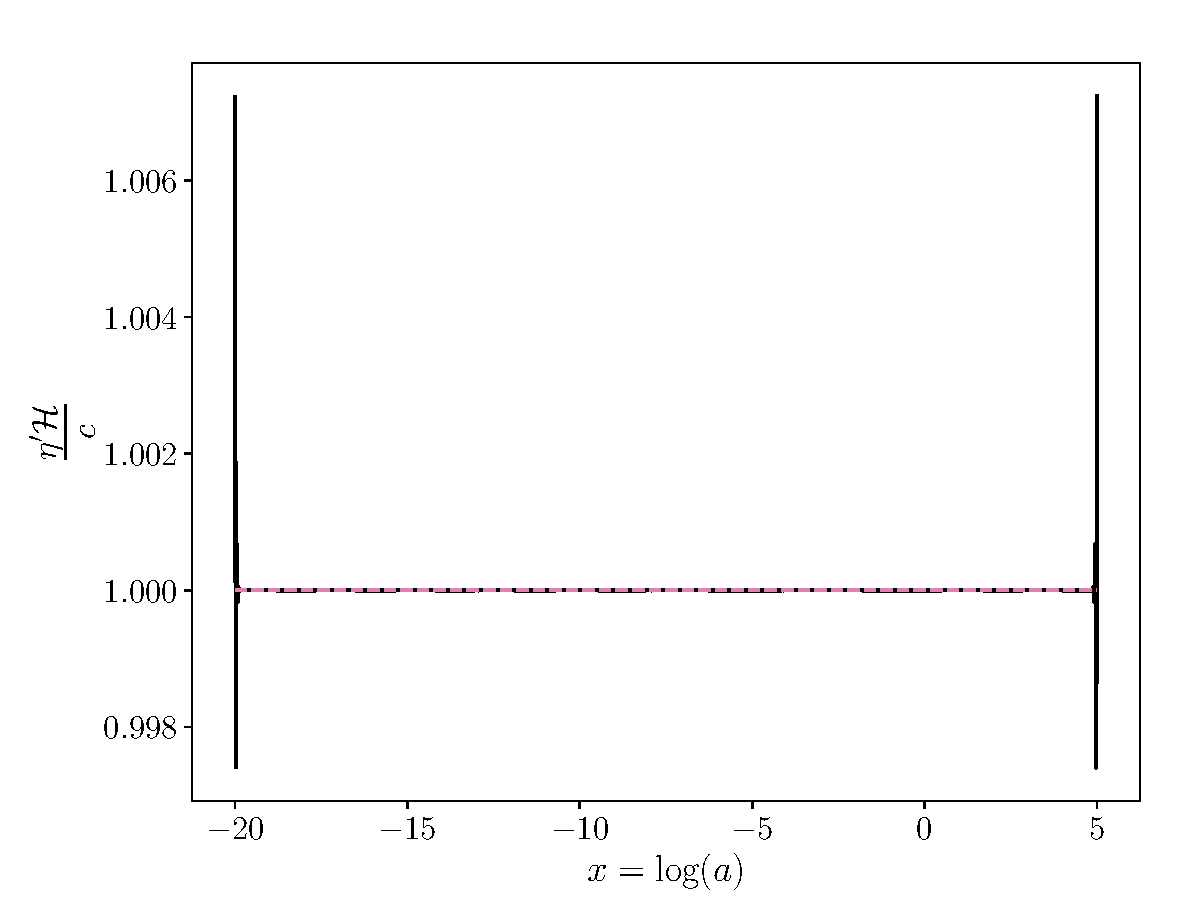
\includegraphics[width=\columnwidth]{/Users/paljettrosa/Documents/GitHub/AST5220/figs/numerical_stability.pdf}
    \caption{\colorbox{Plum}{caption}.}\label{fig:numerical stability}
\end{figure}

\begin{figure*}
    \centering
    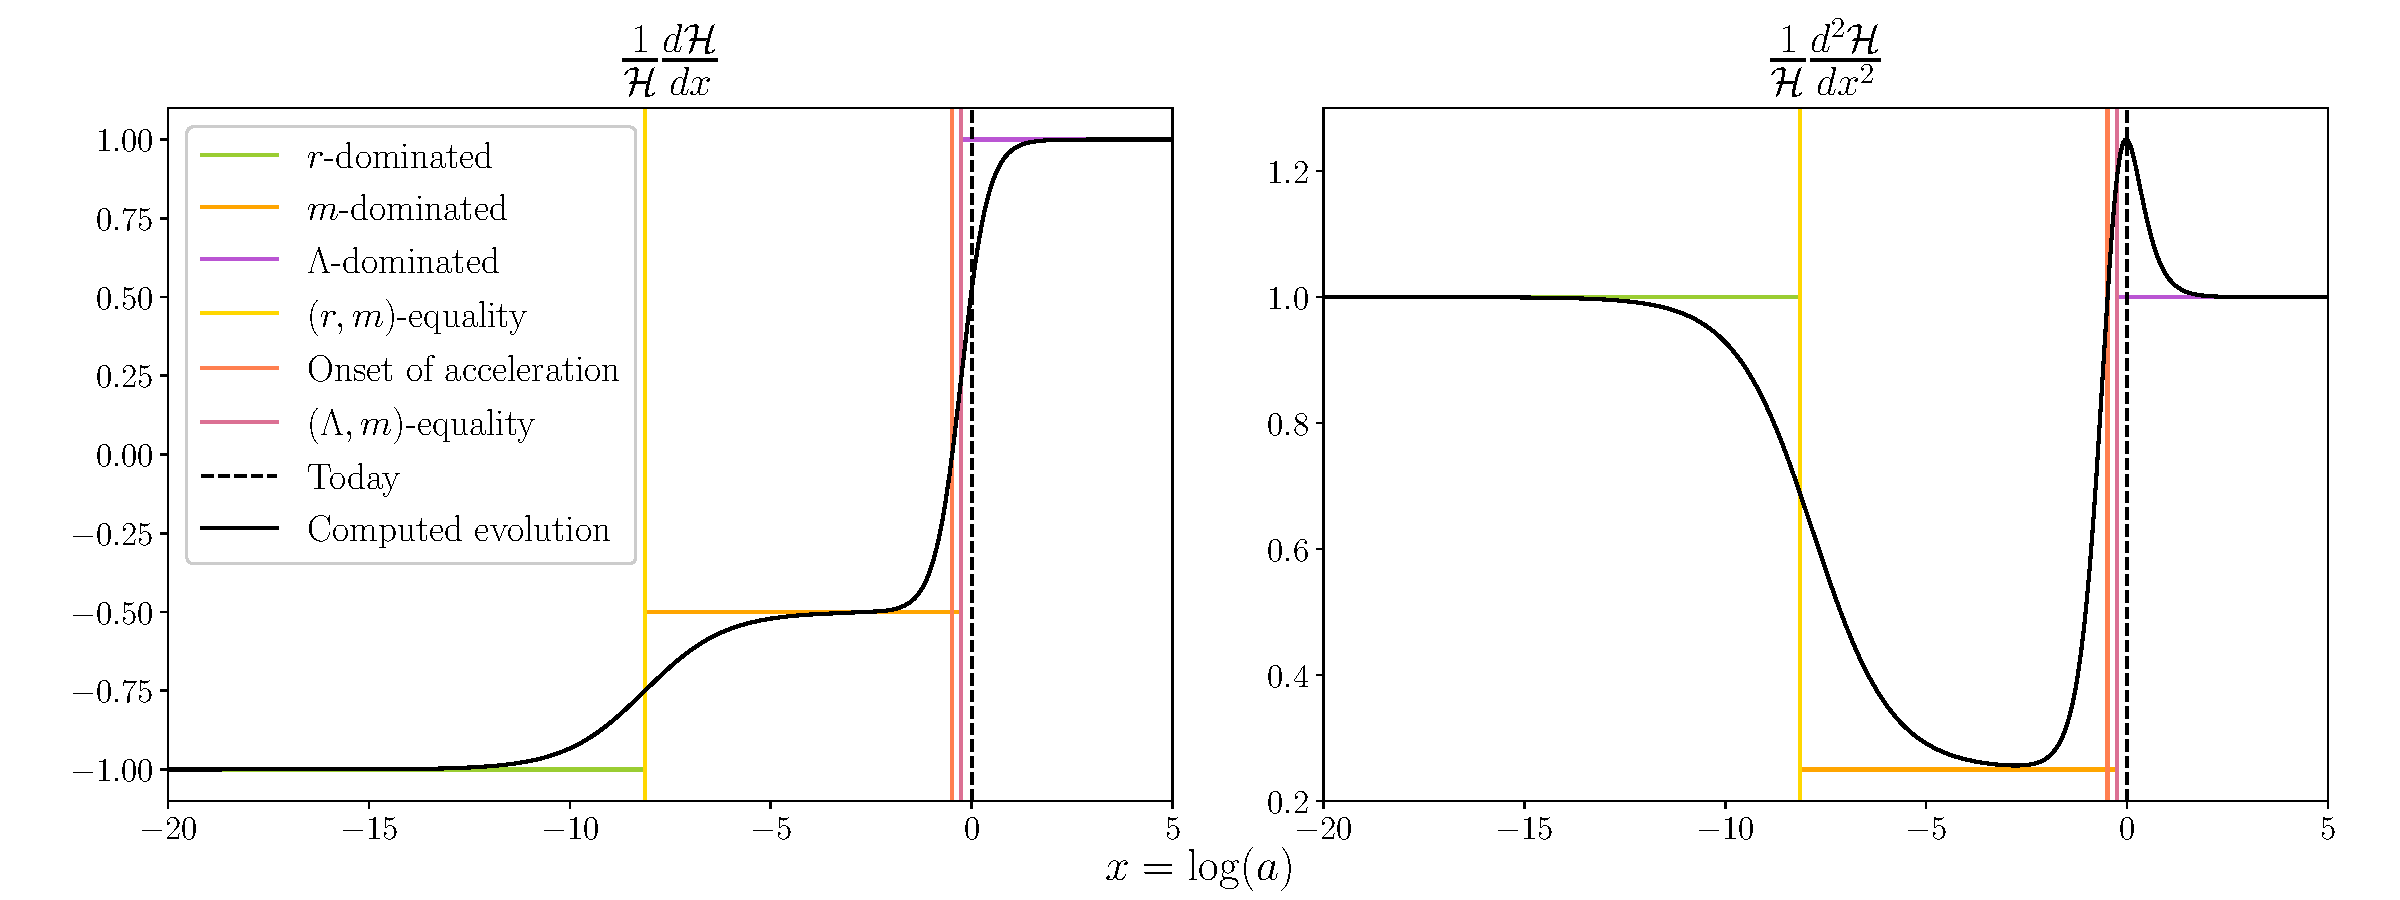
\includegraphics[width=\textwidth]{/Users/paljettrosa/Documents/GitHub/AST5220/figs/H_prime_derivatives.pdf}
    \caption{\colorbox{Plum}{caption}.}\label{fig:H_prime derivatives}
\end{figure*}


\subsubsection{Time evolution}
\colorbox{Plum}{maybe rename / split into fewer sections}

\begin{figure}[h!]
    \centering
    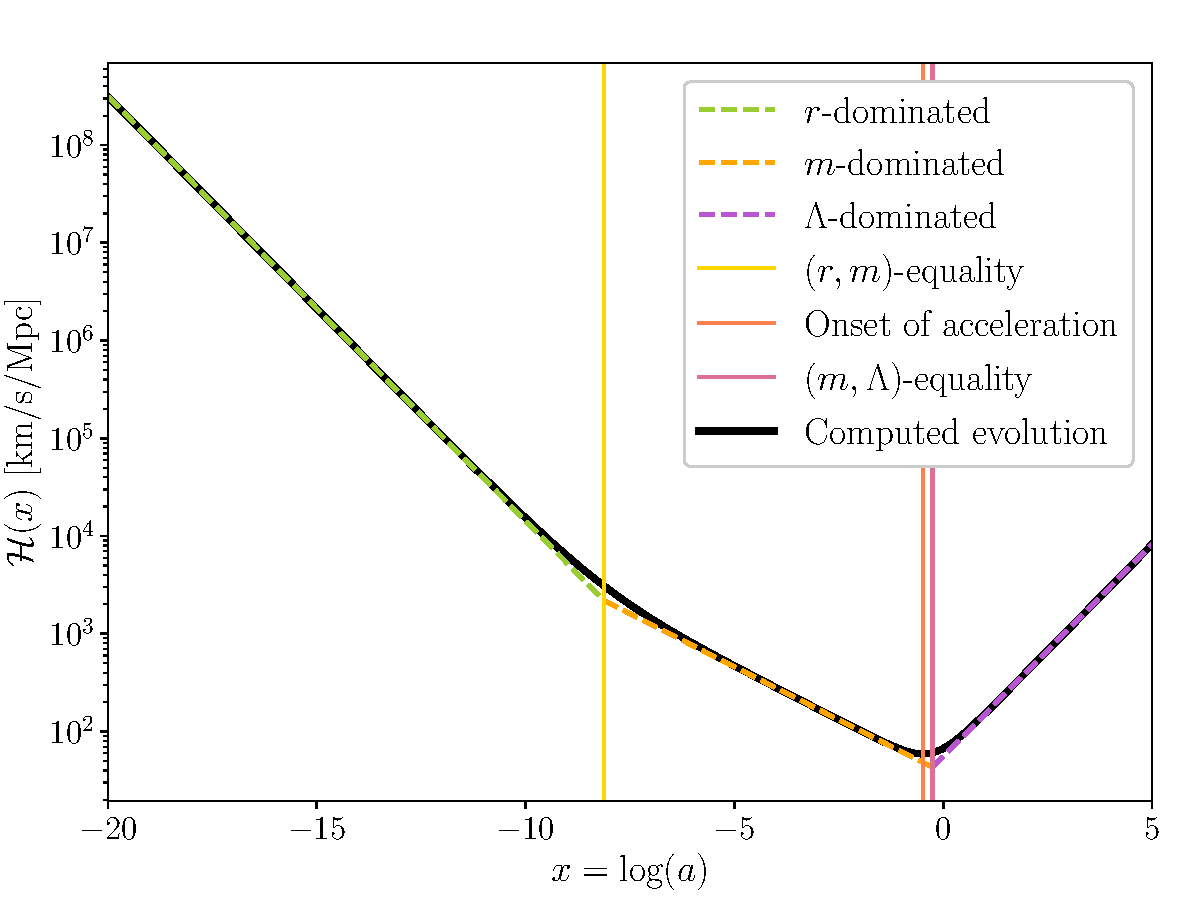
\includegraphics[width=\columnwidth]{/Users/paljettrosa/Documents/GitHub/AST5220/figs/H_prime.pdf}
    \caption{\colorbox{Plum}{caption}.}\label{fig:H_prime}
\end{figure}

\begin{figure*}
    \centering
    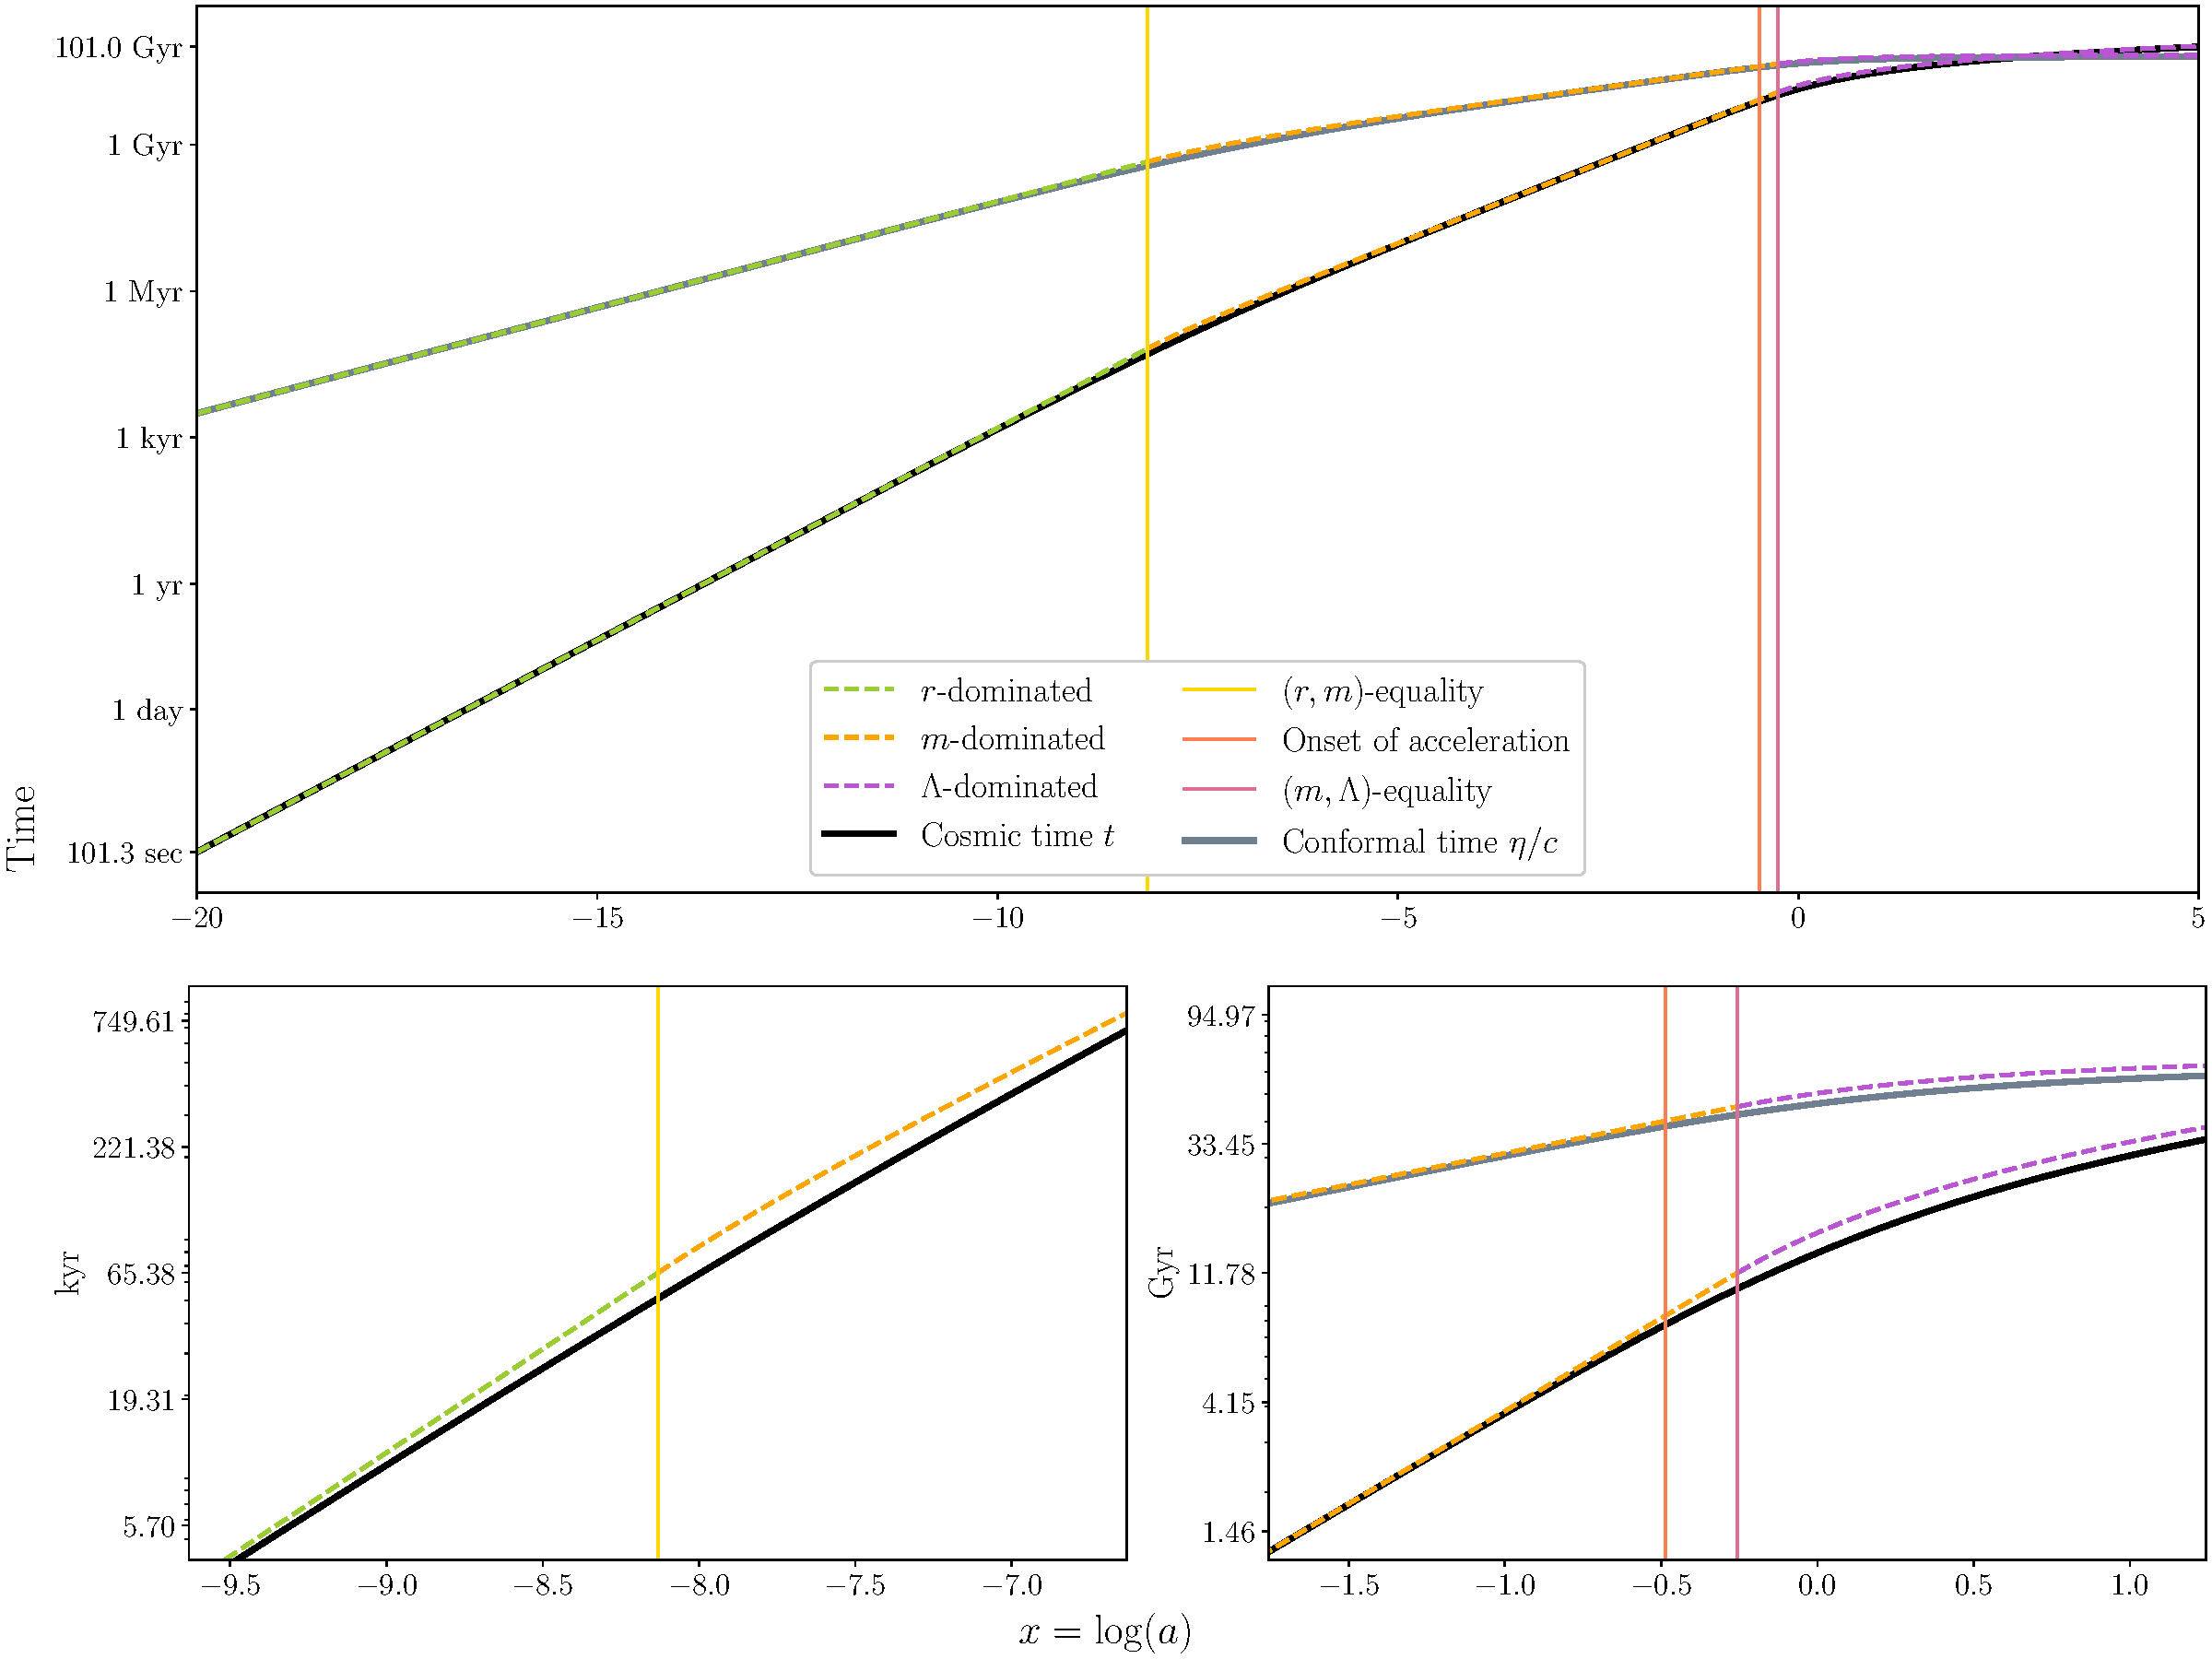
\includegraphics[width=\textwidth]{/Users/paljettrosa/Documents/GitHub/AST5220/figs/eta_and_t.pdf}
    \caption{\colorbox{Plum}{caption}.}\label{fig:eta and t}
\end{figure*}

\begin{figure}[h!]
    \centering
    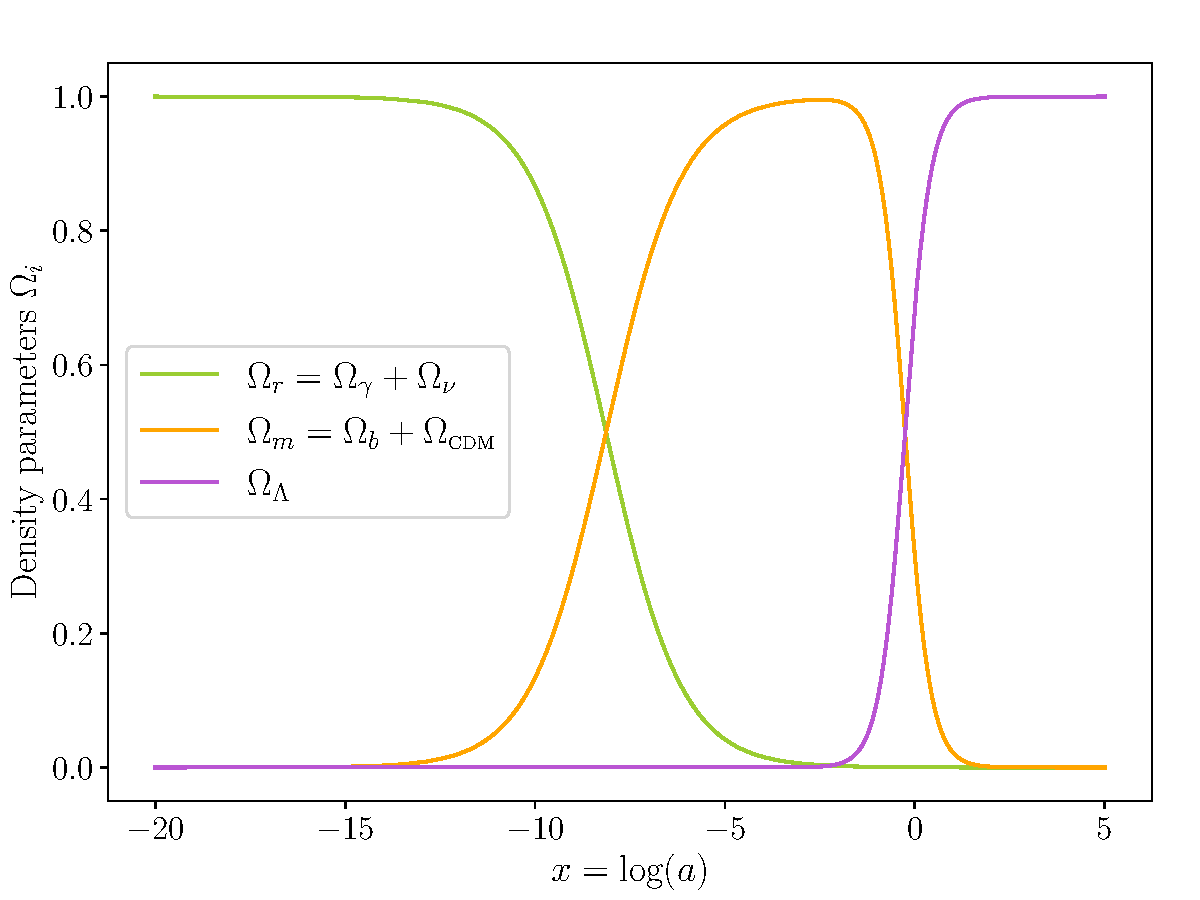
\includegraphics[width=\columnwidth]{/Users/paljettrosa/Documents/GitHub/AST5220/figs/density_parameters.pdf}
    \caption{\colorbox{Plum}{caption}.}\label{fig:density parameters}
\end{figure}



\subsubsection{Supernova fitting}
\begin{figure}[h!]
    \centering
    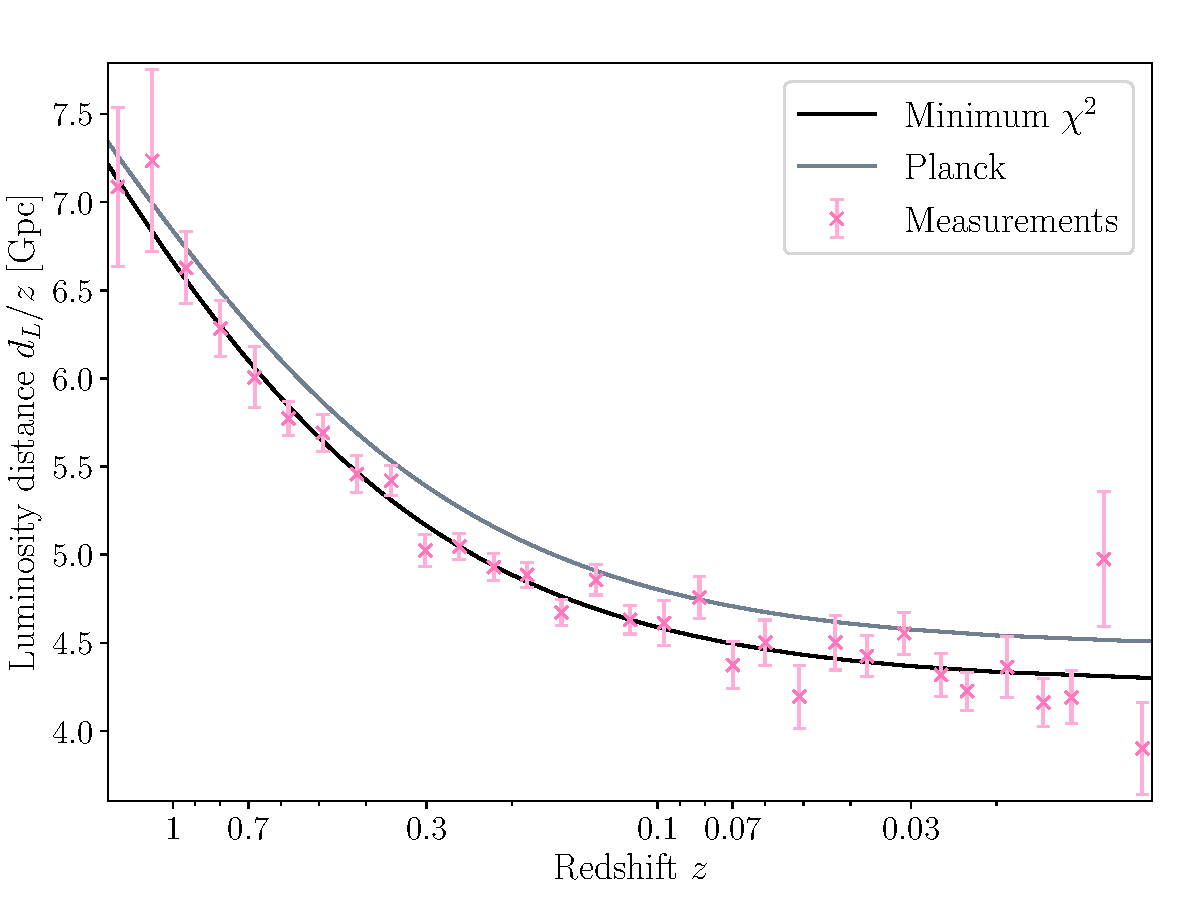
\includegraphics[width=\columnwidth]{/Users/paljettrosa/Documents/GitHub/AST5220/figs/luminosity_distance.pdf}
    \caption{\colorbox{Plum}{caption}.}\label{fig:luminosity distance}
\end{figure}

\begin{figure}[h!]
    \centering
    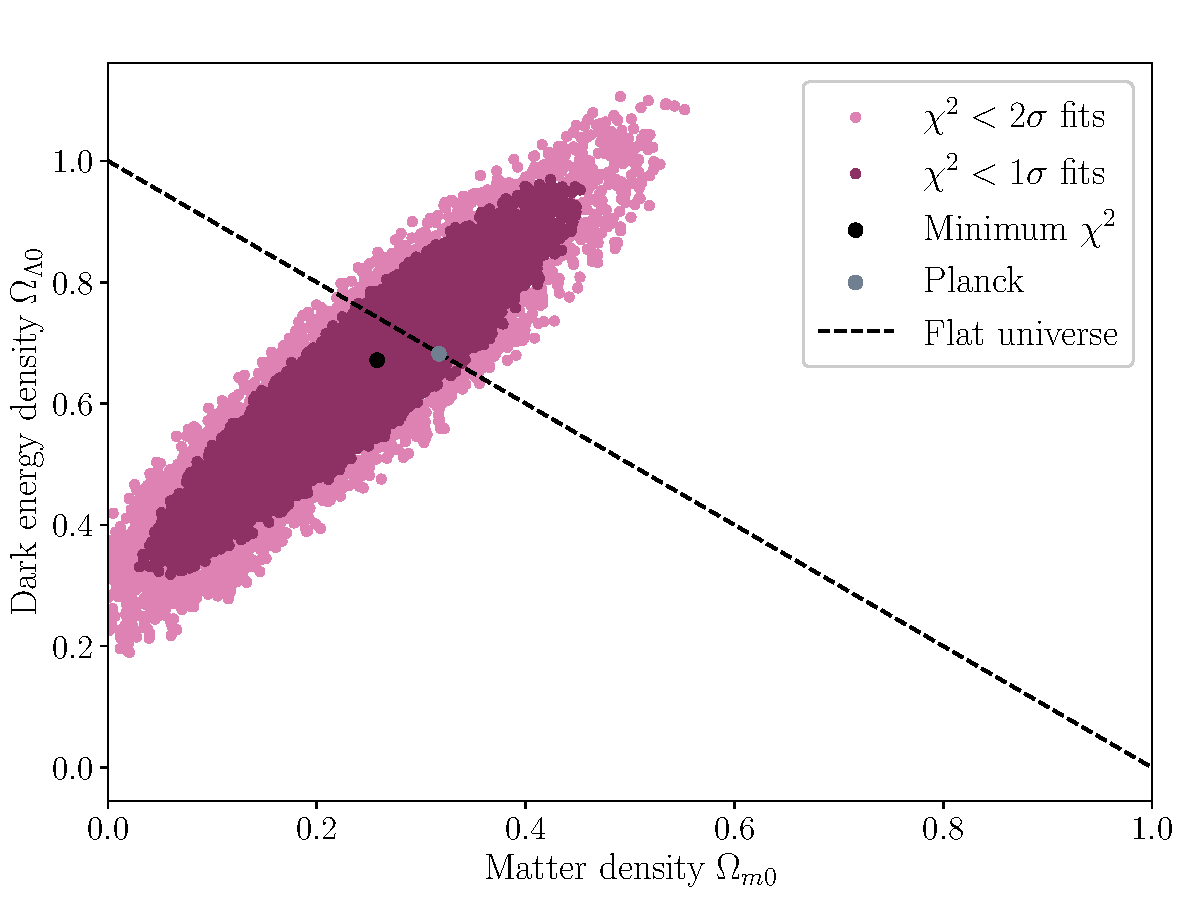
\includegraphics[width=\columnwidth]{/Users/paljettrosa/Documents/GitHub/AST5220/figs/MCMC_fits.pdf}
    \caption{\colorbox{Plum}{caption}.}\label{fig:MCMC fits}
\end{figure}

\begin{figure*}
      \centering
      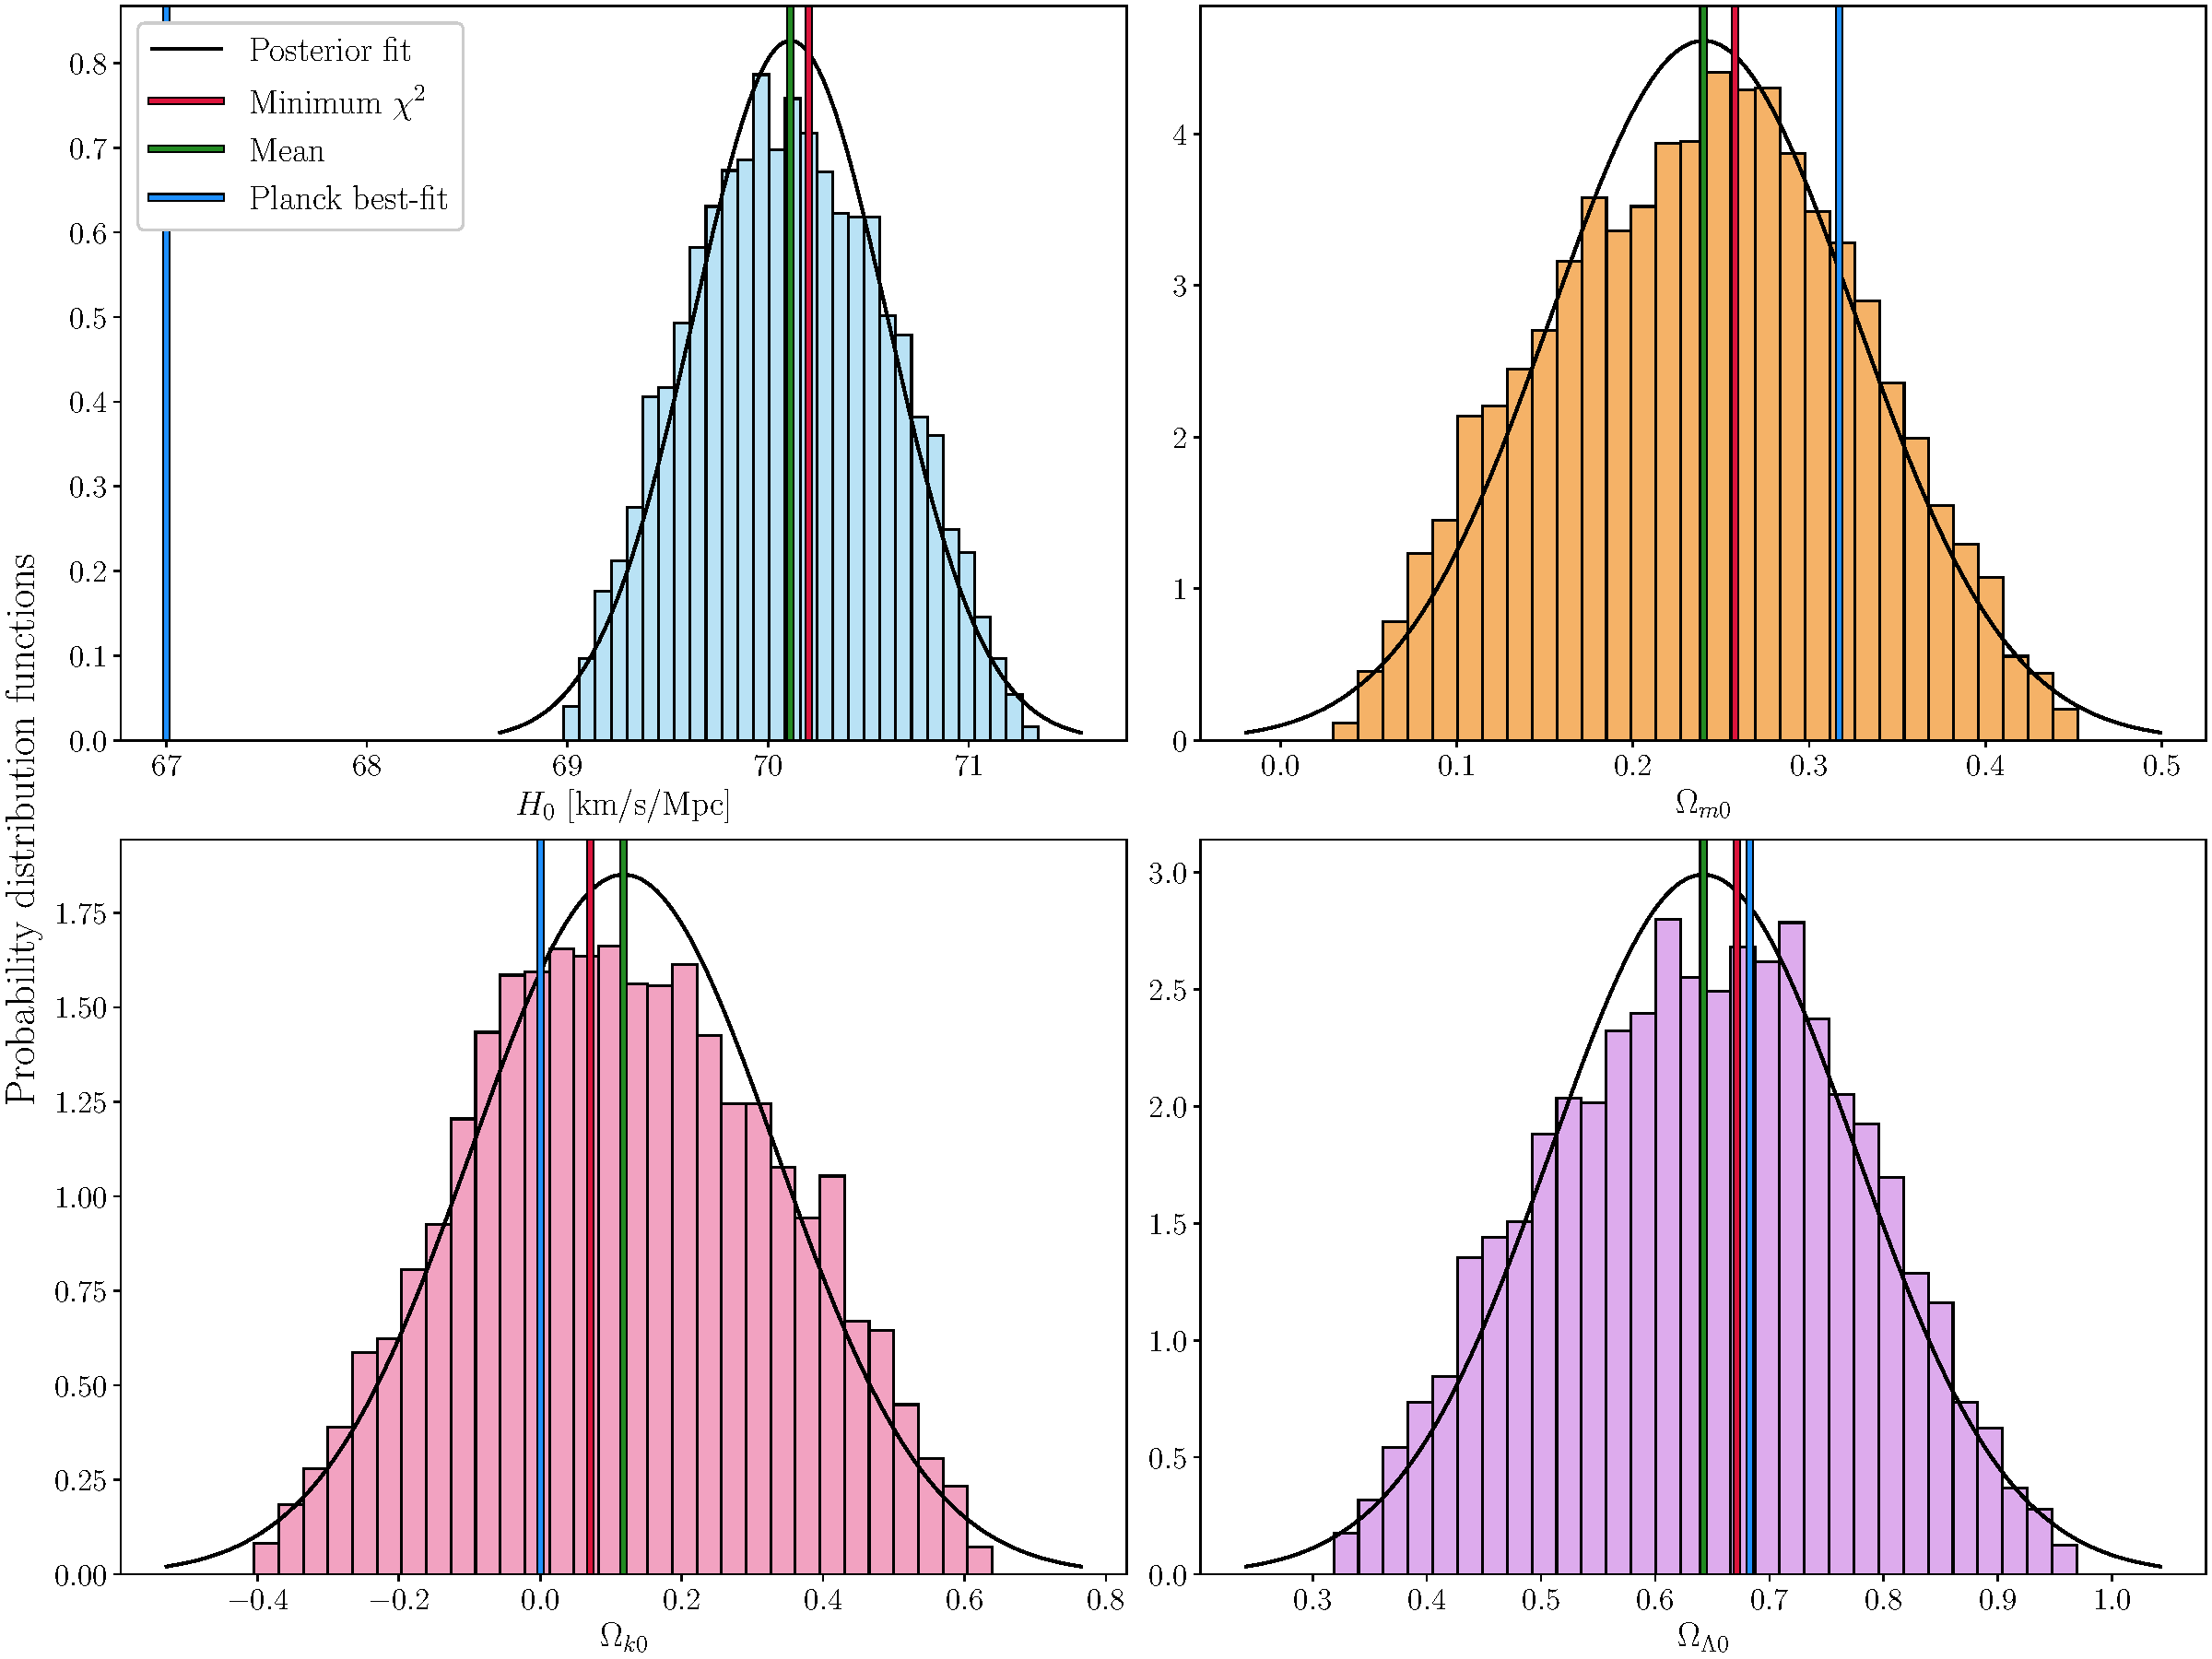
\includegraphics[width=\textwidth]{/Users/paljettrosa/Documents/GitHub/AST5220/figs/distributions.pdf}
      \caption{\colorbox{Plum}{caption}.}\label{fig:distributions}
\end{figure*}



\section{Milestone II}\label{sec: milestone II}

\subsection{Theory}\label{subsec: II theory}

\subsection{Implementation}\label{subsec: II methods}

\subsection{Results}\label{subsec: II results}



\section{Milestone III}\label{sec: milestone III}

\subsection{Theory}\label{subsec: III theory}

\subsection{Implementation}\label{subsec: III methods}

\subsection{Results}\label{subsec: III results}



\section{Milestone IV}\label{sec: milestone IV}

\subsection{Theory}\label{subsec: IV theory}

\subsection{Implementation}\label{subsec: IV methods}

\subsection{Results}\label{subsec: IV results}



\section{Conclusions}\label{sec: conclusions}

\cite{Armadillo}
\bibliographystyle{aa} % style aa.bst
\bibliography{references} % your references Yourfile.bib


\end{document}